% Provenance (never printed): old seconde/premiere S material on the water
% cycle on land (the drainage basin, river discharge, floods and their
% management); see sources/book2/PROVENANCE.md. The Varden basin is computed
% in figdata/grade-10/varden_basin.py from figdata/shared/region.py; the
% Potomac record in figdata/grade-10/flood_frequency.py.
\chapter{Drainage Basins, Rivers and Floods}\label{ch:g10:drainage-basins}

A river can rise two days after the rain has stopped, at a town where no
rain fell at all. The water that floods its streets fell earlier, on hills
far upstream; it ran down their slopes into streams, and the streams joined
into the river that brought it, all at once, to the town. To understand a
flood, one must look beyond the river to the whole area that feeds it, and
follow the water through it. This chapter defines that area, the \omterm{def:g10:drainage-basins:drainage-basin}{drainage
basin}; measures what a river carries, its \omterm{def:g10:drainage-basins:discharge}{discharge}; follows a flood as it
passes a point of the river; and shows how a long record of floods tells how
often a given flood comes back.

\begin{omfigure}
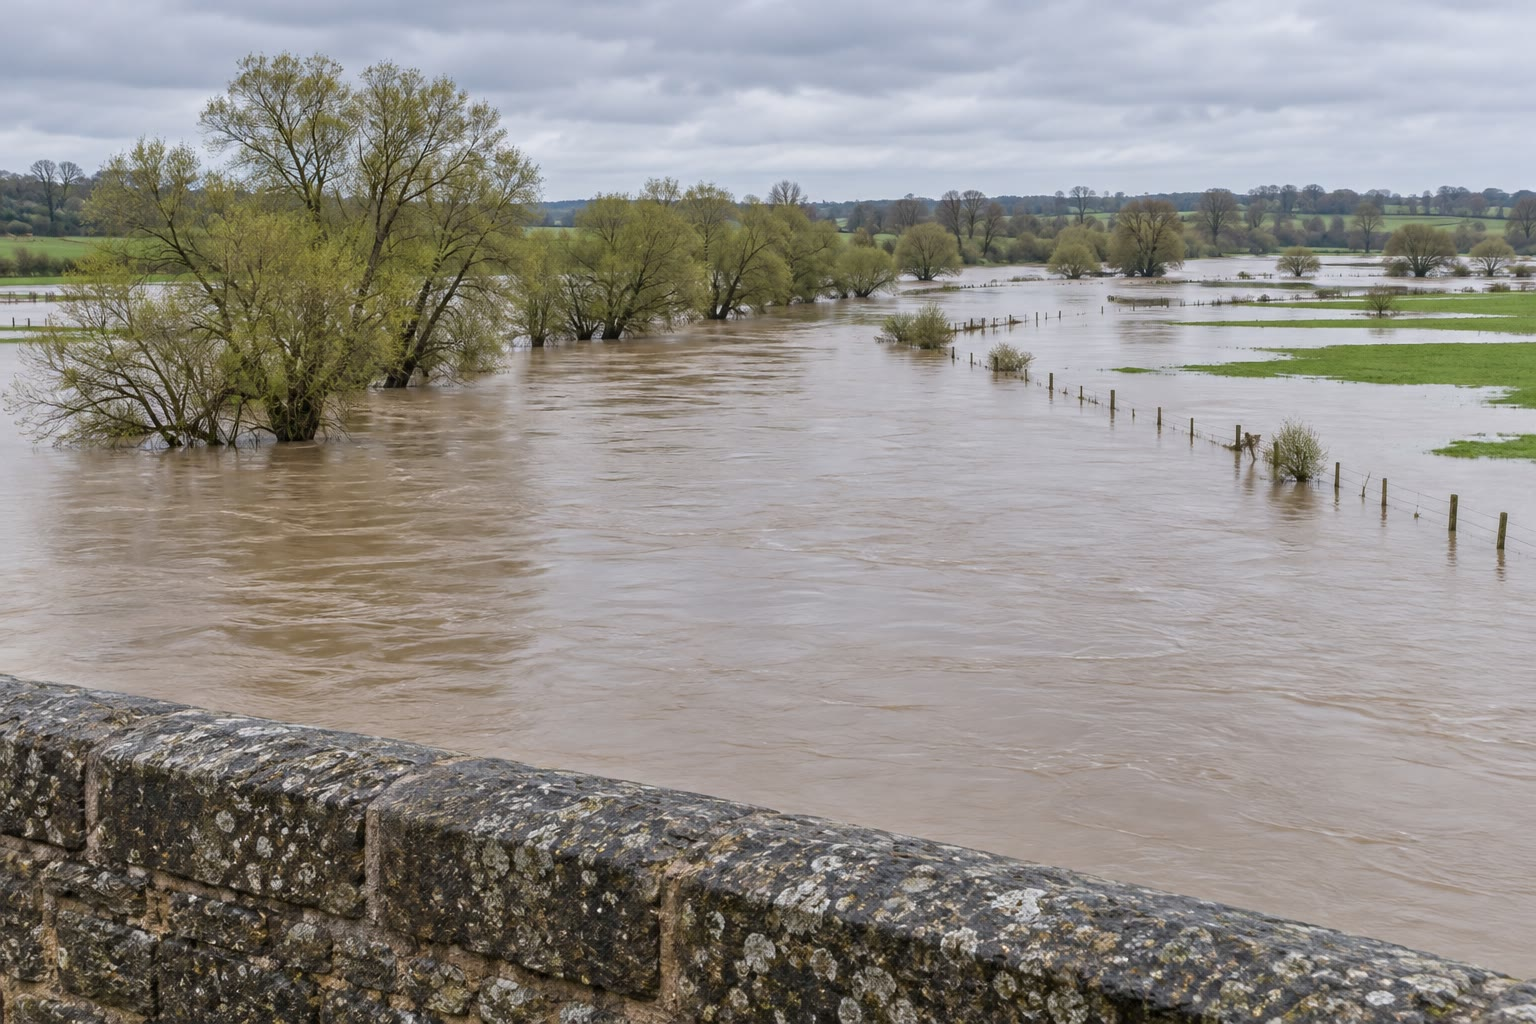
\includegraphics[width=0.8\linewidth]{images/book2/ai/g10-river-flood-meadows.jpg}

{\small A river in flood, seen from a stone bridge: the brown water, loaded
with mud, has left its channel and covers the meadows of its floodplain, up
to the fences and the trees that line its usual banks.}
\end{omfigure}

\begin{recall}
Rain that reaches the ground soaks into it, runs off its surface, or
evaporates; the water cycle carries it back to the sea (the physics books). Water soaks into permeable rocks and fills them below
the water table, forming aquifers that feed springs and rivers (Book 1,
grade 6). A river winds in meanders across its flat floodplain, which it
covers when it floods (Book 1, grade 5). Contour lines join points of equal
height; the Varden Hills are the region drawn on the maps of this series
(Book 1, grades 2 and 9).
\end{recall}

\begin{safety}
Flood water is far more dangerous than it looks. About \qty{15}{cm} of
fast-moving water can knock an adult over, and about \qty{30}{cm} can carry a
car away; the road under it may have collapsed. Never walk or drive into flood
water: turn around and go another way.
% ledger: nws:flood-water
\end{safety}

\section{The drainage basin}

Every drop of rain that does not evaporate or soak in deeply runs downhill.
It follows the steepest slope of the ground, joins a rill, then a stream,
and the streams join into rivers. All the land whose water ends in the same
river forms one unit.

\begin{definition}[Drainage basin; drainage divide]\label{def:g10:drainage-basins:drainage-basin}
The \emph{drainage basin}\index{drainage basin} of a point of a river is
the whole area of land whose runoff flows to the river upstream of that
point and passes that point. The
\emph{drainage divide}\index{drainage divide} is the line that separates two neighbouring drainage basins: it
follows the crests of the land, and the rain falling on either side of it
flows to different rivers.
\end{definition}

A basin is always defined for a point of the river, its \emph{outlet}: the
basin of a river where it reaches the sea is the largest, and every point
upstream has a smaller basin inside it. Two drops falling a metre apart, on
either side of a divide, can end in different rivers and even in different
oceans.

\subsection*{The basin of the Varden river}

A computer finds a \omterm{def:g10:drainage-basins:drainage-basin}{drainage basin} from a map of heights in a few steps. The
map is cut into small squares, \qty{50}{m} on a side here. For each square,
the computer looks at its eight neighbours and sends the water to the one
reached by the steepest downward slope. (Where a small hollow has no lower
neighbour, it is first filled up to the level at which it would overflow, as
a puddle does.) Following these steps from square to square traces the path
of a drop from anywhere on the map. The squares whose drops reach the river
form the basin.

\begin{omfigure}
\begin{tikzpicture}
\begin{axis}[axis equal image, xmin=0, xmax=10, ymin=0, ymax=8, width=0.86\linewidth,
  tick label style={font=\scriptsize}, xlabel={east (km)}, ylabel={north (km)},
  label style={font=\small}, enlargelimits=false]
\addplot[fill=omDef!14, draw=none, even odd rule] table {figdata/out/grade-10-varden_basin-fill.dat};
\addplot[contour, line width=0.25pt, opacity=0.7] table {figdata/out/shared-region-contours.dat};
\addplot[index contour, opacity=0.8] table {figdata/out/shared-region-index-contours.dat};
\addplot[river, line width=1.6pt] table {figdata/out/shared-region-river.dat};
\addplot[omThm, line width=1.4pt, dashed] table {figdata/out/grade-10-varden_basin-divide.dat};
\addplot[omWxRain, line width=0.9pt, -{Stealth[length=5pt]}] table {figdata/out/grade-10-varden_basin-path1.dat};
\addplot[omWxRain, line width=0.9pt, -{Stealth[length=5pt]}] table {figdata/out/grade-10-varden_basin-path2.dat};
\addplot[omWxRain, line width=0.9pt, -{Stealth[length=5pt]}] table {figdata/out/grade-10-varden_basin-path3.dat};
\addplot[omWxRain, line width=0.9pt, -{Stealth[length=5pt]}] table {figdata/out/grade-10-varden_basin-path4.dat};
\fill[omWxRain] (axis cs:2,7.4) circle (2.2pt);
\fill[omWxRain] (axis cs:4,1.8) circle (2.2pt);
\fill[omWxRain] (axis cs:8.6,6.6) circle (2.2pt);
\fill[omWxRain] (axis cs:2.5,0.7) circle (2.2pt);
\node[font=\footnotesize, fill=white, fill opacity=0.85, text opacity=1, inner sep=1.5pt, text=omThm] at (axis cs:6.0,6.75) {divide};
\node[font=\footnotesize, fill=white, fill opacity=0.85, text opacity=1, inner sep=1.5pt, text=omThm] at (axis cs:3.5,1.1) {divide};
\node[font=\footnotesize, fill=white, fill opacity=0.85, text opacity=1, inner sep=1.5pt, align=center] at (axis cs:5.3,7.55) {outside the basin:\\water leaves northwards};
\node[font=\footnotesize, fill=white, fill opacity=0.85, text opacity=1, inner sep=1.5pt, align=right, anchor=east] at (axis cs:9.85,3.35) {outlet};
\draw[-{Stealth[length=6pt]}, line width=1pt, omRiver] (axis cs:9.3,3.7) -- (axis cs:9.95,4.15);
\node[font=\footnotesize, fill=white, fill opacity=0.85, text opacity=1, inner sep=1.5pt] at (axis cs:1.1,4.75) {river};
\end{axis}
\end{tikzpicture}

{\small The \omterm{def:g10:drainage-basins:drainage-basin}{drainage basin} of the Varden river on the map of the Varden
Hills (shaded), computed by sending the water of every square of
\qty{50}{m} down the steepest slope; contours every \qty{50}{m}. The dashed
lines are the divides; the blue lines are the paths of four raindrops (dots).
Two reach the river and flow east to the outlet, where the river leaves the
map; the two others, beyond the divides, leave the map towards other
rivers.}
\end{omfigure}

The basin covers \qty{66}{km^2} of the \qty{80}{km^2} of the map, about
four-fifths of it. In the north the divide follows the crests of the
hills and passes over their summits; beyond them the land slopes away from the river and its
water flows to another valley. In the south-west corner a small area also
drains off the map. The river itself enters the map from the west, so its
full basin is larger: it also takes in the land upstream, beyond the edge of
the map.
% values computed in figdata/grade-10/varden_basin.py (basin_km2 66.19, map_km2 80)

\subsection*{The largest rivers}

Rivers are compared by the area of their basin and by the water they carry.
The largest river in the world by far is the Amazon. The Mississippi, the
largest river of the United States, drains about \num{1150000} square miles,
about 2.98 million \unit{km^2}, from the United States and Canada.
% ledger: kammerer:mississippi

\section{Discharge}

\begin{definition}[Discharge]\label{def:g10:drainage-basins:discharge}
The \emph{discharge}\index{discharge} of a river at a point is the volume of
water that passes through a cross-section of the river in one second. It is
measured in cubic metres per second, \unit{m^3/s}.
\end{definition}

A \omterm{def:g10:drainage-basins:discharge}{discharge} of \qty{1}{m^3/s} is a thousand litres every second, or
\qty{86400}{m^3} a day. The water flows fastest near the surface in the
middle of the channel and slowest along its bed and banks, where it rubs
against them; the \emph{mean velocity} is the velocity averaged over the
whole cross-section.

\begin{proposition}[Discharge, velocity and cross-section]\label{prop:g10:drainage-basins:discharge}
The \omterm{def:g10:drainage-basins:discharge}{discharge} $Q$ of a river is the product of the mean velocity $v$ of the
water and the area $A$ of the wetted cross-section:
\[
Q = v\,A.
\]
\end{proposition}

\begin{proof}
In a time $t$, the water that crosses the section has moved forward by a
distance $v\,t$: it fills a slab of the river of cross-section $A$ and
length $v\,t$, of volume $A\,v\,t$. Dividing this volume by the time $t$
gives the volume per second, $Q = v\,A$.
\end{proof}

A river with a cross-section of \qty{50}{m^2} flowing at a mean velocity of
\qty{1.2}{m/s} carries $1.2 \times 50 = \qty{60}{m^3/s}$. In flood, both
factors grow: the water deepens and widens, so the cross-section grows, and
it flows faster.

\subsection*{Measuring a discharge}

Since the velocity changes across the river, it is measured at several
points. The river is cut into vertical strips; in each, the depth and the
velocity are measured, and the \omterm{def:g10:drainage-basins:discharge}{discharges} of the strips are added.

\begin{method}[The velocity--area method]\label{met:g10:drainage-basins:velocity-area}
\begin{enumerate}
  \item Stretch a measuring tape across the river and choose verticals at
        regular spacings $w$ along it.
  \item At each vertical, measure the depth $d$ and the mean velocity $v$
        of the water over that depth with a current meter.
  \item Each vertical stands for a strip of width $w$ and area $w\,d$; its
        \omterm{def:g10:drainage-basins:discharge}{discharge} is $v\,w\,d$.
  \item Add the \omterm{def:g10:drainage-basins:discharge}{discharges} of all the strips: $Q = \sum v\,w\,d$.
        The cross-section is $A = \sum w\,d$ and the mean velocity $Q/A$.
\end{enumerate}
\end{method}

\begin{omfigure}
\begin{tikzpicture}[x=0.9cm, y=1.6cm, font=\footnotesize]
  % water
  \fill[omSea] (0,0) -- (1,-0.4) -- (2,-0.75) -- (3,-1.0) -- (4,-1.25) -- (5,-1.4) -- (6,-1.3)
     -- (7,-1.1) -- (8,-0.8) -- (9,-0.5) -- (10,-0.2) -- (10.5,0) -- cycle;
  \fill[omDef!22] (4,0) -- (4,-1.25) -- (5,-1.4) -- (6,-1.3) -- (6,0) -- cycle;
  % bed
  \draw[line width=0.9pt, brown!60!black] (-0.6,0.35) -- (0,0) -- (1,-0.4) -- (2,-0.75) -- (3,-1.0) -- (4,-1.25)
     -- (5,-1.4) -- (6,-1.3) -- (7,-1.1) -- (8,-0.8) -- (9,-0.5) -- (10,-0.2) -- (10.5,0) -- (11.1,0.35);
  \draw[omDef!70!black, line width=0.5pt] (0,0) -- (10.5,0);
  % verticals
  \foreach \x/\d/\v/\dx in {1/0.4/0.3/0.3, 3/1.0/0.6/0, 5/1.4/0.8/0, 7/1.1/0.7/0, 9/0.5/0.4/-0.25} {
    \draw[black!70, dashed] (\x,0) -- (\x,-\d);
    \node[anchor=south, font=\scriptsize] at (\x,0.02) {\qty{\v}{m/s}};
    \node[font=\scriptsize, fill=white, inner sep=0.8pt] at (\x+\dx,-0.5*\d) {\qty{\d}{m}};
  }
  \draw[{Stealth}-{Stealth}] (4,0.42) -- node[above, font=\scriptsize] {one strip: $w = \qty{2}{m}$} (6,0.42);
  \node[anchor=west, align=left] at (11.2,-0.15) {water\\surface};
  \node[anchor=west, align=left] at (11.2,-0.9) {bed};
  \draw[black!50] (11.15,-0.9) -- (8.5,-0.68);
  \node[anchor=north] at (5.25,-1.75) {mean velocities measured at the verticals (above the water) and depths (in the water)};
\end{tikzpicture}

{\small Measuring a \omterm{def:g10:drainage-basins:discharge}{discharge} (schematic; vertical scale exaggerated). Five
verticals, \qty{2}{m} apart, divide a stream about \qty{10}{m} wide into
strips; the shaded strip is the one measured at the middle vertical.}
\end{omfigure}

\begin{example}[A gauging]\label{ex:g10:drainage-basins:gauging}
In the stream of the figure, the five strips, each \qty{2}{m} wide, have
areas $2 \times 0.4 = 0.8$, $2.0$, $2.8$, $2.2$ and \qty{1.0}{m^2}: the
cross-section is \qty{8.8}{m^2}. Their \omterm{def:g10:drainage-basins:discharge}{discharges} are $0.3 \times 0.8 =
0.24$, $0.6 \times 2.0 = 1.20$, $0.8 \times 2.8 = 2.24$, $0.7 \times 2.2 =
1.54$ and $0.4 \times 1.0 = \qty{0.40}{m^3/s}$, so the stream carries
$Q \approx \qty{5.6}{m^3/s}$. The mean velocity is $5.62/8.8 \approx
\qty{0.64}{m/s}$, less than the \qty{0.8}{m/s} of the middle of the stream.
\end{example}

\begin{omfigure}
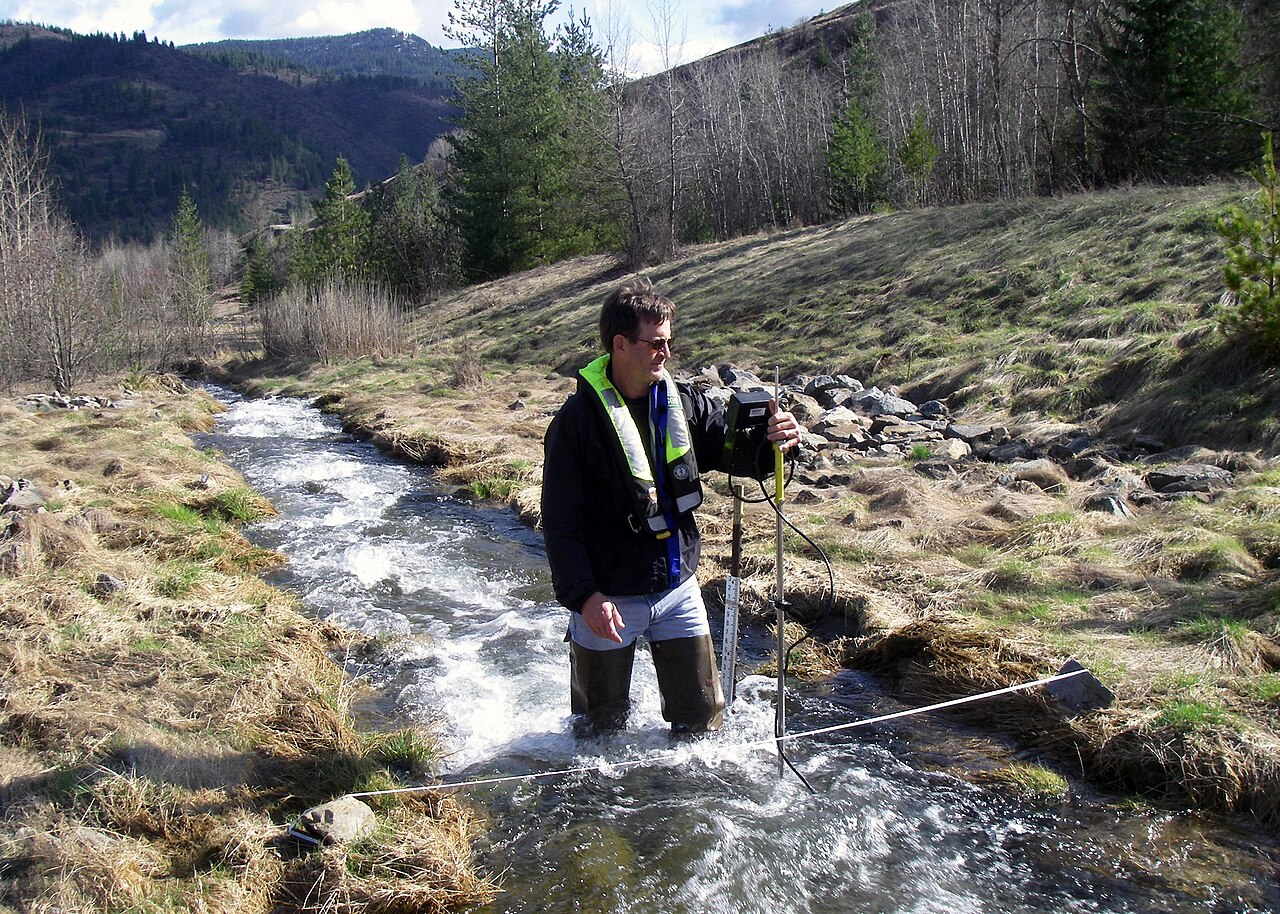
\includegraphics[height=4.6cm]{images/book2/g10-usgs-hydrologist-streamflow.jpg}\hspace{0.3cm}%
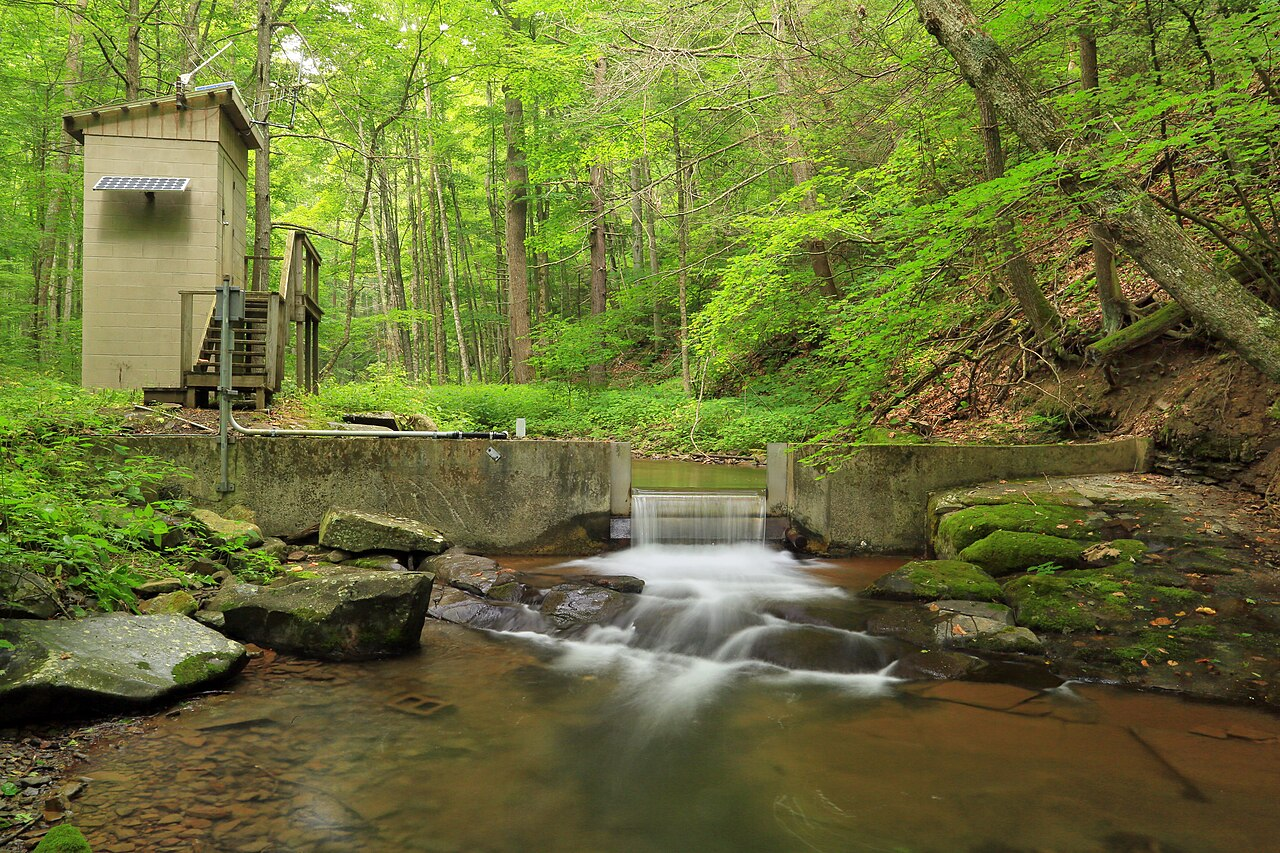
\includegraphics[height=4.6cm]{images/book2/g10-usgs-streamgage.jpg}

{\small Left: a hydrologist measures the \omterm{def:g10:drainage-basins:discharge}{discharge} of a mountain stream by the
velocity--area method; the tape stretched across the stream marks the
verticals, and the rod carries a current meter. Right: a gauging station on
a forest stream; the hut holds the instruments that record the water level
behind the small weir. Photographs: U.S. Geological Survey
(public domain).}
\end{omfigure}

A gauging takes time and cannot be made continuously. A gauging station
records instead the level of the water, without a break. A few
gaugings made at different levels give a curve relating the level to the
\omterm{def:g10:drainage-basins:discharge}{discharge}, and the station turns each level it records into a \omterm{def:g10:drainage-basins:discharge}{discharge}.

Large rivers carry enormous \omterm{def:g10:drainage-basins:discharge}{discharges}. From 1972 to 2003 the Amazon
delivered on average about \qty{206000}{m^3/s} to the Atlantic Ocean, within
about \qty{6}{\percent}: about \qty{17}{\percent} of all the fresh water that
the rivers of the world bring to the sea. The Mississippi brings on average
\num{593000} cubic feet per second, about \qty{16800}{m^3/s}, to the Gulf of
Mexico: the Amazon carries some twelve times more.
% ledger: callede:amazon, kammerer:mississippi

\section{The hydrograph}

\begin{definition}[Hydrograph; baseflow; lag time]\label{def:g10:drainage-basins:hydrograph}
A \emph{hydrograph}\index{hydrograph} is the graph of the \omterm{def:g10:drainage-basins:discharge}{discharge} of a
river at one point against time. The \emph{baseflow}\index{baseflow} is the
part of the \omterm{def:g10:drainage-basins:discharge}{discharge} fed by groundwater, which keeps the river flowing
between rains. The \emph{lag time}\index{lag time} of a flood is the time
between the peak of the rainfall on the basin and the peak of the \omterm{def:g10:drainage-basins:discharge}{discharge}.
\end{definition}

\begin{omfigure}
\begin{tikzpicture}[x=1cm, y=1cm, font=\footnotesize]
  \draw[-{Stealth}] (0,0) -- (10.2,0) node[below left] {time};
  \draw[-{Stealth}] (0,0) -- (0,5.9) node[above right] {discharge};
  % rain bars hanging from the top
  \draw[black!50] (0,5.4) -- (10,5.4);
  \foreach \x/\h in {1.0/0.15, 1.3/0.35, 1.6/0.55, 1.9/0.4, 2.2/0.2} {
    \fill[omWxRain!70] (\x,5.4) rectangle ++(0.28,-\h);
  }
  \node[anchor=south west] at (2.6,5.4) {rainfall on the basin};
  % baseflow and hydrograph
  \fill[omSea] (0,0.7) -- (2.0,0.7) .. controls (2.8,0.8) and (3.3,3.3) .. (4.0,3.6)
    .. controls (4.6,3.6) and (5.1,2.1) .. (6.0,1.55) .. controls (7.0,1.0) and (8.0,0.85) .. (10,0.8)
    -- (10,0) -- (0,0) -- cycle;
  \fill[omLithAlluv] (0,0) -- (0,0.7) -- (2.0,0.7) .. controls (3.5,0.68) and (5.5,0.75) .. (6.6,0.95)
    .. controls (8,1.0) and (9,0.85) .. (10,0.8) -- (10,0) -- cycle;
  \draw[omDef, line width=1.2pt] (0,0.7) -- (2.0,0.7) .. controls (2.8,0.8) and (3.3,3.3) .. (4.0,3.6)
    .. controls (4.6,3.6) and (5.1,2.1) .. (6.0,1.55) .. controls (7.0,1.0) and (8.0,0.85) .. (10,0.8);
  \draw[black!60, dashed] (2.0,0.7) .. controls (3.5,0.68) and (5.5,0.75) .. (6.6,0.95);
  % lag time
  \draw[black!60, densely dotted] (1.74,4.85) -- (1.74,4.3);
  \draw[black!60, densely dotted] (3.98,3.65) -- (3.98,4.3);
  \draw[{Stealth}-{Stealth}] (1.74,4.3) -- node[above] {lag time} (3.98,4.3);
  % labels
  \node[anchor=west] at (4.2,3.75) {peak};
  \node[anchor=east, align=right] at (2.9,2.2) {rising\\limb};
  \node[anchor=west, align=left] at (5.4,2.3) {falling limb};
  \node[align=center] at (4.5,1.25) {runoff};
  \node at (8.2,0.4) {baseflow};
\end{tikzpicture}

{\small The \omterm{def:g10:drainage-basins:hydrograph}{hydrograph} of a flood (schematic). After the rain, the \omterm{def:g10:drainage-basins:discharge}{discharge}
rises to a peak and falls back more slowly; the area under the curve is the
volume of water. The \omterm{def:g10:drainage-basins:hydrograph}{baseflow}, fed by groundwater, changes little; the rest
is the runoff that the rain sent quickly to the river.}
\end{omfigure}

The water of a storm reaches the river at different times. Rain falling near
the channel arrives within minutes or hours; rain falling far upstream takes
much longer, since it must flow down the slopes and along the river. The
\omterm{def:g10:drainage-basins:discharge}{discharge} therefore rises steeply, on the \emph{rising limb}, while the water
of the nearby slopes arrives, peaks when the most water arrives at once, and
falls more slowly, on the \emph{falling limb}, as the last water drains from
the far corners of the basin and from the soil. The larger the basin, the
longer the \omterm{def:g10:drainage-basins:hydrograph}{lag time}: hours for a small stream, days for a large river.

Some basins give \emph{flashy} floods, with a high, sudden peak and a short
\omterm{def:g10:drainage-basins:hydrograph}{lag time}; others give slow, flat floods. The same rain gives a flashier flood
when:
\begin{itemize}
  \item the basin is small and steep, so that the water has a short, fast
        way to go;
  \item the ground lets little water soak in: bare rock, clay, ground that is
        already soaked, frozen ground, and above all the roofs, roads and car
        parks of a town, which send almost all the rain straight into drains
        and streams;
  \item the basin has a dense network of streams and drains, which collects
        the water quickly.
\end{itemize}
Forests, deep permeable soils and wide floodplains do the opposite: they hold
the water back and release it slowly, which lowers and delays the peak.

\subsection*{A real flood}

The Potomac River drains a basin of \num{11560} square miles, about
\qty{29900}{km^2}, upstream of a gauging station near Washington, in the
eastern United States. In January 1996 the station recorded the \omterm{def:g10:drainage-basins:hydrograph}{hydrograph}
below.
% ledger: data:b2-usgs-potomac

\begin{omfigure}
\begin{tikzpicture}
\begin{axis}[omrecord, width=0.86\linewidth, height=6cm, xmin=0, xmax=55, ymin=0, ymax=10000,
  xtick={0,10,20,30,40,50}, xticklabels={5 Jan, 15 Jan, 25 Jan, 4 Feb, 14 Feb, 24 Feb},
  ylabel={discharge (\unit{m^3/s})}, xlabel={1996},
  tick label style={font=\small}, label style={font=\small},
  scaled y ticks=false, yticklabel style={/pgf/number format/fixed}]
\addplot[omDef, line width=1.1pt, mark=*, mark size=1.1pt] table[x=day, y=q] {figdata/out/grade-10-flood_frequency-hydrograph.dat};
\node[anchor=west, font=\footnotesize] at (axis cs:17,9231) {\qty{9231}{m^3/s} on 21 January};
\draw[black!60, dashed] (axis cs:5,334) -- (axis cs:13,334);
\node[anchor=south, font=\footnotesize] at (axis cs:9,1000) {about \qty{330}{m^3/s}};
\draw[black!60] (axis cs:9,1000) -- (axis cs:9,390);
\end{axis}
\end{tikzpicture}

{\small Daily mean \omterm{def:g10:drainage-basins:discharge}{discharge} of the Potomac River near Washington from
5 January to 29 February 1996: the flood rose from \qty{362}{m^3/s} on 18 January
to more than \qty{9000}{m^3/s} three days later, then fell back over the
following weeks, with a smaller second rise at the end of January. Data: U.S.
Geological Survey, station 01646500.}
\end{omfigure}
% values computed in figdata/grade-10/flood_frequency.py (hydro_peak_m3s 9231, hydro_before_mean 334)

In the days before the flood the river carried about \qty{330}{m^3/s}, its
\omterm{def:g10:drainage-basins:hydrograph}{baseflow}. On 21 January the daily mean reached \qty{9231}{m^3/s}, almost
thirty times more. Spread over the whole basin, the water passing the
station that day would make a layer
$9231 \times 86400 / (29\,900 \times 10^6) \approx \qty{0.027}{m}$, about
\qty{27}{mm} deep: a heavy fall of rain, delivered in one day from the whole
basin at once.
% ledger: data:b2-usgs-potomac (hydro_peak_mm_per_day 26.6 in figdata/grade-10/flood_frequency.py)

\section{Floods and their return period}

How large a flood should a town expect? The answer comes from the past: a
gauging station that has run for decades has recorded the largest \omterm{def:g10:drainage-basins:discharge}{discharge}
of every year, the \emph{annual peak}. Small peaks come almost every year,
large ones rarely. The rarer a flood, the larger it is.

\begin{definition}[Return period]\label{def:g10:drainage-basins:return-period}
The \emph{return period}\index{return period} $T$ of a flood is the average
interval, in years, between years whose annual peak equals or exceeds it. A
flood of return period $T$, a \emph{$T$-year flood}, has a probability $1/T$
of being equalled or exceeded in any one year.
\end{definition}

A hundred-year flood is not a flood that comes once every hundred years, like
a timetable. It is a flood that has one chance in a hundred of being equalled
or exceeded each year, every year, whatever happened the year before. Two can
come in successive years; a century can pass without one.

\begin{method}[Return periods from a record of annual peaks]\label{met:g10:drainage-basins:return-periods}
\begin{enumerate}
  \item List the annual peaks of $n$ years.
  \item Rank them from the largest (rank $m = 1$) to the smallest
        (rank $m = n$).
  \item Give the peak of rank $m$ the \omterm{def:g10:drainage-basins:return-period}{return period} $T = (n + 1)/m$.
  \item Plot the peaks against $T$ on a logarithmic scale of $T$, and read
        the \omterm{def:g10:drainage-basins:discharge}{discharge} for the \omterm{def:g10:drainage-basins:return-period}{return period} wanted.
\end{enumerate}
\end{method}

The largest of $n$ peaks thus gets $T = n + 1$ years: in a record of
\num{95} years, \num{96} years. The formula reflects what the record shows:
the peak of rank $m$ has been equalled or exceeded in $m$ of the $n$ years,
about once every $n/m$ years. The method cannot reliably reach beyond the
length of the record: a \num{50}-year record says little about the
\num{1000}-year flood.

\begin{omfigure}
\begin{tikzpicture}
\begin{axis}[omrecord, width=0.86\linewidth, height=6.2cm, xmode=log, xmin=0.9, xmax=150,
  ymin=0, ymax=15000, xlabel={return period $T$ (years)}, ylabel={annual peak (\unit{m^3/s})},
  xtick={1,2,5,10,20,50,100}, xticklabels={1,2,5,10,20,50,100},
  tick label style={font=\small}, label style={font=\small},
  scaled y ticks=false, yticklabel style={/pgf/number format/fixed}]
\addplot[only marks, mark=*, mark size=1.5pt, omDef] table[x=T, y=peak] {figdata/out/grade-10-flood_frequency-ranked.dat};
\node[anchor=east, font=\footnotesize] at (axis cs:92,13705) {1936};
\node[anchor=east, font=\footnotesize] at (axis cs:46,12658) {1942};
\node[anchor=south, font=\footnotesize] at (axis cs:32,10300) {1972};
\node[anchor=north west, font=\footnotesize, align=left] at (axis cs:1.1,14000) {Potomac River near Washington,\\annual peaks 1931--2025 ($n = 95$)};
\end{axis}
\end{tikzpicture}

{\small The \num{95} annual peaks of the Potomac River near Washington, ranked
and plotted against their \omterm{def:g10:drainage-basins:return-period}{return periods} $T = (n+1)/m$. The largest, in March
1936, gets $T = 96$ years. Data: U.S. Geological Survey, station 01646500.}
\end{omfigure}
% values computed in figdata/grade-10/flood_frequency.py

\begin{dated}{2026}
In the record of the Potomac near Washington, from 1931 to 2025, the five
largest annual peaks came in March 1936 (\qty{13700}{m^3/s}), October 1942,
June 1972, April 1937 and January 1996, the last two equal at
\qty{9830}{m^3/s}.
% ledger: data:b2-usgs-potomac
\end{dated}

\subsection*{The chance of a flood over many years}

A house or a bridge stands for decades. What matters to it is not the chance
of a flood in one year, but over its whole life.

\begin{proposition}[At least one flood in $N$ years]\label{prop:g10:drainage-basins:chance}
If the years are independent of one another, the probability that a flood of
\omterm{def:g10:drainage-basins:return-period}{return period} $T$ is equalled or exceeded at least once in $N$ years is
\[
P = 1 - \left(1 - \frac{1}{T}\right)^{N}.
\]
\end{proposition}

\begin{proof}
In one year, the probability that the flood does \emph{not} happen is
$1 - 1/T$. The years being independent, the probability that it happens in
none of $N$ years is the product of $N$ such factors, $(1 - 1/T)^N$. The
event ``at least once'' is the opposite of ``never'', so its probability is
$1 - (1 - 1/T)^N$.
\end{proof}

For a hundred-year flood over thirty years, $(0.99)^{30} \approx 0.740$, and
$P \approx 0.26$: one chance in four. Over a hundred years, $(0.99)^{100}
\approx 0.366$ and $P \approx 0.63$: the hundred-year flood is far from
certain to come in a hundred years.

\begin{omfigure}
\begin{tikzpicture}
\begin{axis}[omrecord, width=0.82\linewidth, height=5.8cm, xmin=0, xmax=100, ymin=0, ymax=1,
  xlabel={number of years $N$}, ylabel={chance of at least one flood},
  ytick={0,0.2,0.4,0.6,0.8,1}, yticklabels={0, 20\,\%, 40\,\%, 60\,\%, 80\,\%, 100\,\%},
  tick label style={font=\small}, label style={font=\small},
  legend pos=south east, legend style={font=\footnotesize}]
\addplot[omThm, line width=1pt] table[x=n, y=p10] {figdata/out/grade-10-flood_frequency-chance.dat};
\addplot[omProp, line width=1pt] table[x=n, y=p50] {figdata/out/grade-10-flood_frequency-chance.dat};
\addplot[omDef, line width=1pt] table[x=n, y=p100] {figdata/out/grade-10-flood_frequency-chance.dat};
\legend{{10-year flood}, {50-year flood}, {100-year flood}}
\draw[black!60, dashed] (axis cs:30,0) -- (axis cs:30,0.2603) -- (axis cs:0,0.2603);
\fill[omDef] (axis cs:30,0.2603) circle (2pt);
\node[anchor=north west, font=\footnotesize] at (axis cs:31,0.22) {26\,\% in 30 years};
\end{axis}
\end{tikzpicture}

{\small The chance that a flood of \omterm{def:g10:drainage-basins:return-period}{return period} 10, 50 or 100 years comes at
least once in $N$ years.}
\end{omfigure}
% values computed in figdata/grade-10/flood_frequency.py (chance_100_30 0.2603)

\section{Dams and levees}

People have long built structures that change how a flood passes. Two
change it in opposite ways.

A \emph{dam} holds back a reservoir. When a flood arrives, part of its water
is stored in the reservoir, whose level rises, and is released afterwards,
over a longer time. Downstream, the same volume of water passes, but spread
out: the peak is lower and later. A reservoir lowers a flood only as long as
it has room left; once full, all the water that enters it passes on.

A \emph{levee} is a bank of earth built along a river to keep its floods off
the floodplain. Between the levees the water cannot spread out; to carry the
same \omterm{def:g10:drainage-basins:discharge}{discharge} through the narrower section, it must stand higher and flow
faster. The land behind the levees stays dry, as long as the levees hold and
are not overtopped. But the floodplain no longer stores water during the
flood, so more of it, and sooner, travels downstream.

\begin{omfigure}
\begin{tikzpicture}[x=0.62cm, y=0.62cm, font=\footnotesize]
  \begin{scope}
    \draw[-{Stealth}] (0,0) -- (9.4,0) node[below left] {time};
    \draw[-{Stealth}] (0,0) -- (0,6.0) node[above right] {discharge};
    \draw[omDef, line width=1.2pt] (0,0.6) -- (1,0.6) .. controls (1.8,0.7) and (2.2,5.2) .. (2.8,5.2)
      .. controls (3.5,5.2) and (4,1.6) .. (5,1.0) .. controls (6,0.7) and (7.5,0.6) .. (9,0.6);
    \draw[omThm, line width=1.2pt, dashed] (0,0.6) -- (1.3,0.6) .. controls (2.3,0.75) and (3.0,3.3) .. (3.8,3.3)
      .. controls (4.7,3.3) and (5.8,1.5) .. (6.8,1.0) .. controls (7.6,0.75) and (8.3,0.65) .. (9,0.6);
    \node[anchor=west, text=omDef] at (3.0,5.35) {into the reservoir};
    \node[anchor=west, text=omThm] at (4.2,3.55) {below the dam};
    \node[anchor=north] at (4.5,-0.45) {(a) a dam: lower, later peak};
  \end{scope}
  \begin{scope}[xshift=7.2cm]
    \fill[omLithAlluv] (0,0) -- (10,0) -- (10,1.8) -- (0,1.8) -- cycle;
    \fill[white] (3.5,1.8) -- (3.9,0.4) -- (6.1,0.4) -- (6.5,1.8) -- cycle;
    \fill[omSea] (0.4,2.3) -- (3.25,2.3) -- (3.5,1.8) -- (3.9,0.4) -- (6.1,0.4) -- (6.5,1.8) -- (6.75,2.3) -- (9.6,2.3) -- (9.6,1.8) -- (0.4,1.8) -- cycle;
    \draw[line width=0.8pt, brown!60!black] (0,1.8) -- (3.5,1.8) -- (3.9,0.4) -- (6.1,0.4) -- (6.5,1.8) -- (10,1.8);
    \draw[omDef!70!black] (0.4,2.3) -- (9.6,2.3);
    \node[anchor=south, text=omDef!70!black, align=center] at (1.5,2.35) {without\\levees};
    % levees
    \fill[brown!45] (2.6,1.8) -- (3.0,3.9) -- (3.3,3.9) -- (3.5,1.8) -- cycle;
    \fill[brown!45] (6.5,1.8) -- (6.7,3.9) -- (7.0,3.9) -- (7.4,1.8) -- cycle;
    \fill[omSea!70!omDef] (3.5,1.8) -- (3.9,0.4) -- (6.1,0.4) -- (6.5,1.8) -- (6.65,3.4) -- (3.35,3.4) -- cycle;
    \draw[omThm, line width=0.8pt, dashed] (3.35,3.4) -- (6.65,3.4);
    \node[anchor=south, text=omThm] at (5,3.95) {with levees};
    \draw[omThm] (5,3.95) -- (5,3.45);
    \node[anchor=north] at (5,-0.45) {(b) levees: the flood stands higher};
  \end{scope}
\end{tikzpicture}

{\small Schematic. (a) A reservoir stores part of a flood and releases it
later: below the dam the peak is lower and comes later. (b) Without levees
the flood spreads thinly over the floodplain; between levees the same
\omterm{def:g10:drainage-basins:discharge}{discharge} must pass through a narrow section and stands much higher.}
\end{omfigure}

\section{Exercises}

\begin{exercise}[$\star$]\label{exo:g10:drainage-basins:1}
Define a \omterm{def:g10:drainage-basins:drainage-basin}{drainage basin} and a \omterm{def:g10:drainage-basins:drainage-basin}{drainage divide}. Why can two raindrops falling
a metre apart end in two different seas?
\end{exercise}

\begin{exercise}[$\star$]\label{exo:g10:drainage-basins:2}
Define the \omterm{def:g10:drainage-basins:discharge}{discharge} of a river and give its unit. How many litres pass a
point of a river carrying \qty{1}{m^3/s} in one day?
\end{exercise}

\begin{exercise}[$\star$]\label{exo:g10:drainage-basins:3}
On the \omterm{def:g10:drainage-basins:hydrograph}{hydrograph} of the Potomac in January 1996, read the \omterm{def:g10:drainage-basins:hydrograph}{baseflow} before
the flood, the peak \omterm{def:g10:drainage-basins:discharge}{discharge} and its date, and the number of days the rise
took.
\end{exercise}

\begin{exercise}[$\star$]\label{exo:g10:drainage-basins:4}
What is the probability that a \num{50}-year flood is equalled or exceeded
next year? A \num{50}-year flood came last year: is it less likely this
year?
\end{exercise}

\begin{exercise}[$\star$]\label{exo:g10:drainage-basins:5}
The Mississippi brings on average \num{593000} cubic feet of water per
second to the sea (\num{1}~foot = \qty{0.3048}{m}). Convert this \omterm{def:g10:drainage-basins:discharge}{discharge}
to \unit{m^3/s}, and compare it with the \qty{206000}{m^3/s} of the
Amazon.
\end{exercise}

\begin{exercise}[$\star\star$]\label{exo:g10:drainage-basins:6}
A hydrologist gauges a stream with four verticals \qty{1.5}{m} apart. The
depths are \num{0.3}, \num{0.6}, \num{0.7} and \qty{0.4}{m}; the mean
velocities \num{0.2}, \num{0.5}, \num{0.6} and \qty{0.3}{m/s}. Compute the
cross-section, the \omterm{def:g10:drainage-basins:discharge}{discharge} and the mean velocity.
\end{exercise}

\begin{exercise}[$\star\star$]\label{exo:g10:drainage-basins:7}
A storm drops \qty{20}{mm} of rain over the whole basin of the Varden river
on the map, \qty{66}{km^2}. What volume of water is that? If all of it
reached the outlet over two days, what would be the mean extra \omterm{def:g10:drainage-basins:discharge}{discharge}?
\end{exercise}

\begin{exercise}[$\star\star$]\label{exo:g10:drainage-basins:8}
The annual peaks of a small river over nine years are, in \unit{m^3/s}:
\num{42}, \num{65}, \num{38}, \num{120}, \num{51}, \num{47}, \num{88},
\num{35}, \num{59}. Rank them and give the \omterm{def:g10:drainage-basins:return-period}{return periods} of the three
largest. What is the \omterm{def:g10:drainage-basins:return-period}{return period} of the median peak?
\end{exercise}

\begin{exercise}[$\star\star$]\label{exo:g10:drainage-basins:9}
The same storm falls on two basins of the same area: one steep, covered by
a town, the other gently sloping and forested. Sketch their two \omterm{def:g10:drainage-basins:hydrograph}{hydrographs}
on the same axes and explain the differences.
\end{exercise}

\begin{exercise}[$\star\star$]\label{exo:g10:drainage-basins:10}
At the peak of 21 January 1996, the Potomac carried \qty{9231}{m^3/s} from a
basin of \qty{29900}{km^2}. What depth of water, spread over the whole
basin, does one day of this \omterm{def:g10:drainage-basins:discharge}{discharge} represent? Compare with the \omterm{def:g10:drainage-basins:hydrograph}{baseflow} of
\qty{330}{m^3/s}.
\end{exercise}

\begin{exercise}[$\star\star$]\label{exo:g10:drainage-basins:11}
What is the probability that a \num{10}-year flood comes at least once in
\num{10} years? That it does not come at all in these ten years?
\end{exercise}

\begin{exercise}[$\star\star\star$]\label{exo:g10:drainage-basins:12}
The \omterm{def:g10:drainage-basins:discharge}{discharge} entering a reservoir in a flood rises steadily from
\qty{0}{m^3/s} to \qty{1200}{m^3/s} in one day, then falls steadily back to
\qty{0}{m^3/s} in two days (\omterm{def:g10:drainage-basins:hydrograph}{baseflow} neglected). What volume does the flood
bring? The dam lets at most \qty{800}{m^3/s} through, and the reservoir can
store \num{60} million \unit{m^3}. Can it hold back everything above
\qty{800}{m^3/s}?
\end{exercise}

\begin{exercise}[$\star\star\star$]\label{exo:g10:drainage-basins:13}
A river \qty{100}{m} wide is full to its banks at \qty{800}{m^3/s}, flowing
at \qty{2}{m/s}. A flood of \qty{1200}{m^3/s} arrives.
\begin{enumerate}
  \item Without levees, the extra \qty{400}{m^3/s} spreads over a floodplain
        \qty{900}{m} wide, where it flows at \qty{0.5}{m/s}. How deep is the
        water on the floodplain?
  \item With levees, all the flood passes between them, at \qty{2}{m/s}.
        How deep is the river, and how far above its banks does it stand?
\end{enumerate}
\end{exercise}

\begin{exercise}[$\star\star\star$]\label{exo:g10:drainage-basins:14}
What \omterm{def:g10:drainage-basins:return-period}{return period} $T$ gives a flood a chance of one in two of coming at
least once in \num{30} years?
\end{exercise}

\begin{exercise}[$\star\star\star$]\label{exo:g10:drainage-basins:15}
A small map is cut into squares of \qty{100}{m}; their heights in metres are
given below (north at the top). Water leaves each square towards the lowest
of its four neighbours (north, south, east, west) if it is lower; the squares
at \qty{34}{m} (north-west corner) and \qty{30}{m} (south-east corner) are the
outlets of two streams.
\begin{center}
\begin{tabular}{|c|c|c|c|}
\hline
34 & 38 & 46 & 50 \\ \hline
37 & 42 & 48 & 47 \\ \hline
45 & 49 & 44 & 39 \\ \hline
51 & 46 & 37 & 30 \\ \hline
\end{tabular}
\end{center}
Draw the direction of flow of each square, find the basin of each outlet and
its area, and draw the divide.
\end{exercise}

\section{Problem: The Hundred-Year Flood}

\begin{problem}[{Weekend problem --- how often does the river come into town?}]
\label{pb:g10:drainage-basins:1}
% ledger: data:b2-usgs-potomac (values computed in figdata/grade-10/flood_frequency.py)
Imagine a town on the Potomac River, just upstream of Washington, near a
gauging station that has recorded the river's largest \omterm{def:g10:drainage-basins:discharge}{discharge} every year
since 1931. The annual peaks are drawn below, with the \omterm{def:g10:drainage-basins:hydrograph}{hydrograph} of
January 1996 given in the chapter.

\begin{center}
\begin{tikzpicture}
\begin{axis}[omrecord, width=0.9\linewidth, height=5.4cm, ybar, bar width=1.6pt, xmin=1929, xmax=2027,
  ymin=0, ymax=15000, ylabel={annual peak (\unit{m^3/s})}, xlabel={year},
  xtick={1930,1950,1970,1990,2010}, xticklabel style={/pgf/number format/1000 sep={}},
  tick label style={font=\small}, label style={font=\small},
  scaled y ticks=false, yticklabel style={/pgf/number format/fixed}]
\addplot[fill=omDef!70, draw=none] table[x=year, y=peak] {figdata/out/grade-10-flood_frequency-record.dat};
\draw[omThm, dashed] (axis cs:1929,9500) -- (axis cs:2027,9500);
\node[anchor=south east, font=\footnotesize, text=omThm] at (axis cs:2026,9500) {\qty{9500}{m^3/s}};
\end{axis}
\end{tikzpicture}

{\small Annual peak \omterm{def:g10:drainage-basins:discharge}{discharges} of the Potomac River near Washington, water
years 1931--2025 (a water year runs from October to September: the flood of
October 1942 counts in 1943). Data: U.S. Geological Survey, station 01646500.}
\end{center}

\medskip
\noindent\textbf{Part I --- The basin and the discharge.}
\begin{enumerate}
  \item The station's basin covers \num{11560} square miles
        (\num{1}~mile = \qty{1.609}{km}). Convert this area to
        \unit{km^2}.
  \item What line on a map bounds this area?
  \item The largest peak, on 19 March 1936, was \num{484000} cubic feet per
        second. Convert it to \unit{m^3/s} (\num{1}~foot =
        \qty{0.3048}{m}).
  \item The median annual peak is \qty{3341}{m^3/s}. How many times larger
        than the median was the flood of 1936?
  \item Suppose that at the peak of 1936 the river was \qty{400}{m} wide and
        \qty{8}{m} deep on average at the station. What would its mean
        velocity have been?
\end{enumerate}

\medskip
\noindent\textbf{Part II --- Reading the flood of 1996.}
\begin{enumerate}[resume]
  \item On the \omterm{def:g10:drainage-basins:hydrograph}{hydrograph} of January 1996, what was the \omterm{def:g10:drainage-basins:hydrograph}{baseflow} in the
        days before the flood?
  \item What was the peak daily \omterm{def:g10:drainage-basins:discharge}{discharge}, and on what day?
  \item How many days did the rise take, from \qty{362}{m^3/s} on
        18 January to the peak?
  \item What depth of water over the whole basin did the peak day carry
        past the station?
  \item A second, smaller rise peaks on 29 January. What does it tell about
        the water reaching the basin?
  \item The \omterm{def:g10:drainage-basins:discharge}{discharge} was back near \qty{410}{m^3/s} on 7 February. How
        long after the peak was that? Why does the falling limb last longer
        than the rising limb?
\end{enumerate}

\medskip
\noindent\textbf{Part III --- Ranking the floods.}
\begin{enumerate}[resume]
  \item The record holds $n = 95$ annual peaks. What \omterm{def:g10:drainage-basins:return-period}{return period} does the
        method give to the largest?
  \item The peak of October 1942 (\qty{12658}{m^3/s}) ranks second. What is
        its \omterm{def:g10:drainage-basins:return-period}{return period}?
  \item The peak of June 1972 (\qty{10166}{m^3/s}) ranks third. What is its
        \omterm{def:g10:drainage-basins:return-period}{return period}?
  \item The floods of April 1937 and January 1996 were equal
        (\qty{9826}{m^3/s}). Given ranks 4 and 5, what \omterm{def:g10:drainage-basins:return-period}{return periods} do they
        get? Does sharing a value matter much here?
  \item On the bar chart, count the years whose peak exceeded
        \qty{9500}{m^3/s}. Estimate the chance of such a peak in any one
        year, and its \omterm{def:g10:drainage-basins:return-period}{return period}.
\end{enumerate}

\medskip
\noindent\textbf{Part IV --- The chance of a flood.}
\begin{enumerate}[resume]
  \item What is the probability that a \num{100}-year flood is equalled or
        exceeded in a given year?
  \item What is the probability that it is not, in that year?
  \item What is the probability that it does not come in \num{30} years,
        the time a family might live in a house by the river?
  \item What is the chance of at least one \num{100}-year flood in
        \num{30} years?
\end{enumerate}
\end{problem}
